\ifx\fulldocument\undefined
\documentclass[aspectratio=169]{beamer}
% \usetheme{sdr}
\graphicspath{{./tex/imgs/}}

\usepackage[utf8]{inputenc}

\title{Programmiamo Umanoidi!}
\subtitle{}
\author{Lorenzo Leonardini}
\institute{Scuola di Robotica}
\date{\today}

\begin{document}

\begin{frame}
	\titlepage
\end{frame}

\section{Che cos'è NAO}
\subsection{Caratteristiche}
\subsection{Movimento}
\subsection{Utilizzi}
\subsection{Software}

\AtBeginSection[]
{
\begin{frame}{Indice}
\tableofcontents[currentsection]
\end{frame}
}
\fi


\section{Choregraphe}

\begin{frame}
\frametitle{Choregraphe}
\begin{columns}
	\column{0.5\textwidth}
		\onslide<1->{Software proprietario di Aldebaran per il controllo dei loro robot}

		\onslide<2->{Creazione di animazioni, dialoghi, Behavior}

		\onslide<3->{Controllo e monitoraggio del robot}
	\column{0.5\textwidth}
		\begin{figure}[ht]
		\begin{center}
		
\includegraphics[width=.7\textwidth]{choregraphe_logo}<1->
		\end{center}
		\end{figure}
\end{columns}
\end{frame}

\begin{frame}
\frametitle{Choregraphe}
\begin{columns}
	\column{0.5\textwidth}
		Pro:
		\begin{itemize}
			\item<2-> Piuttosto inutitivo
			\item<3-> Programmazione a blocchi
			\item<4-> Espandibile tramite Python
			\item<5-> Robot simulato
		\end{itemize}
		Contro:
		\begin{itemize}
			\item<6-> Robot simulato
			\item<7-> \textbf{BUG, CRASH}
			\item<8-> \textbf{SEMPRE} problemi di connessione al robot
		\end{itemize}
	\column{0.5\textwidth}
		\begin{figure}[ht]
		\begin{center}
		
\includegraphics[width=.7\textwidth]{choregraphe_logo}<1->
		\end{center}
		\end{figure}
\end{columns}
\end{frame}

\begin{frame}
\frametitle{Choregraphe}
\begin{figure}[ht]
\begin{center}
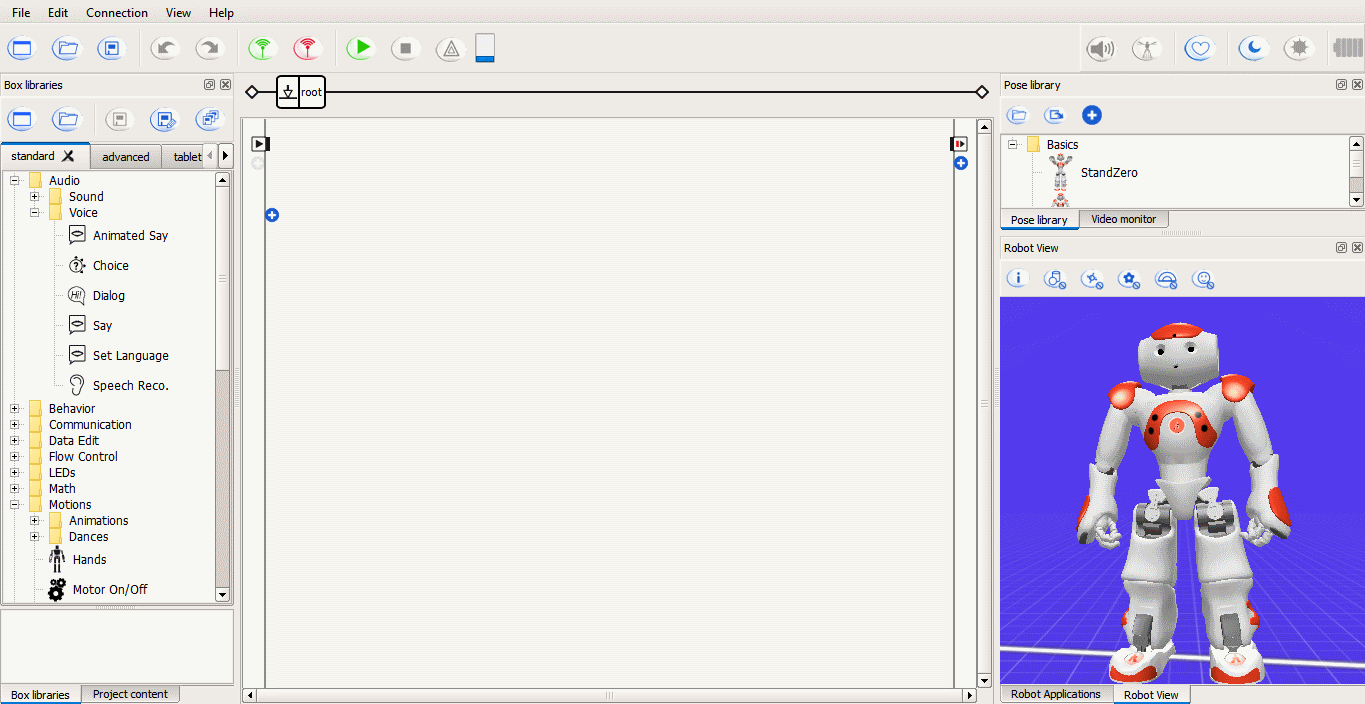
\includegraphics[width=.8\textwidth]{choregraphe.png}
~\footnote{Interfaccia di Choregraphe}
\end{center}
\end{figure}
\end{frame}

\begin{frame}
\frametitle{Choregraphe}
\begin{columns}
	\column{0.5\textwidth}
		\begin{itemize}
			\item<1-> Nella Robot View si può vedere in diretta la posizione del robot
			\item<2-> Si possono manualmente controllare i motori
		\end{itemize}
	\column{0.5\textwidth}
		\begin{figure}[ht]
		\begin{center}
		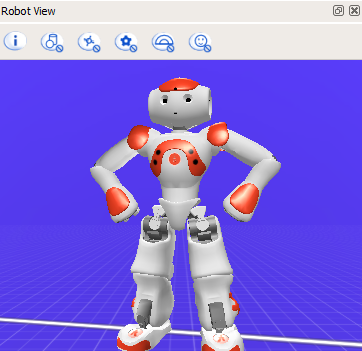
\includegraphics[width=.7\textwidth]{view}<1->
		\end{center}
		\end{figure}
\end{columns}
\end{frame}

\begin{frame}
\frametitle{Choregraphe}
\begin{columns}
	\column{0.5\textwidth}
		\begin{figure}[ht]
		\begin{center}
		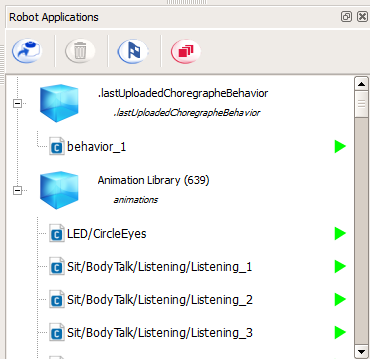
\includegraphics[width=.7\textwidth]{applications}<1->
		\end{center}
		\end{figure}
	\column{0.5\textwidth}
		\begin{itemize}
			\item<1-> Lista completa dei Behavior installati sul robot
			\item<2-> I Behavior si possono creare, modificare, installare e lanciare da Choregraphe
		\end{itemize}
\end{columns}
\end{frame}

\begin{frame}
\frametitle{Choregraphe}
\begin{columns}
	\column{0.5\textwidth}
		\begin{itemize}
			\item<1-> Parte centrale dell'interfaccia
			\item<2-> I blocchi si collegano tramite dei "fili"
			\item<3-> I fili possono essere sdoppiati
		\end{itemize}
	\column{0.5\textwidth}
		\begin{figure}[ht]
		\begin{center}
		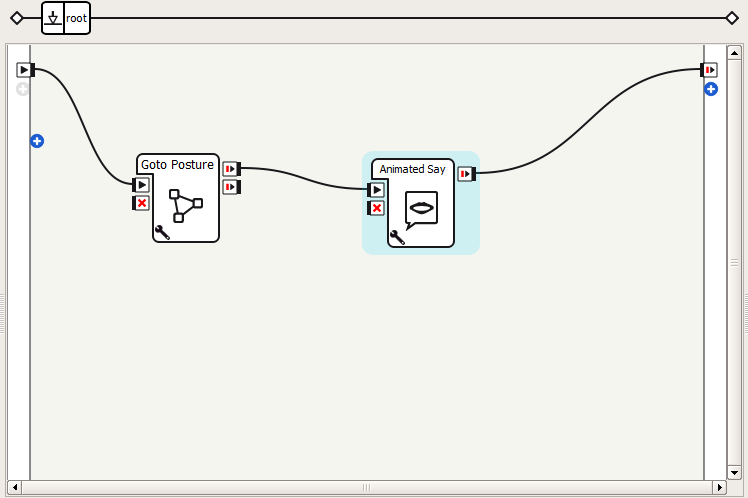
\includegraphics[width=1\textwidth]{blocks}<1->
		\end{center}
		\end{figure}
\end{columns}
\end{frame}

\begin{frame}
\frametitle{Choregraphe}
\begin{columns}
	\column{0.5\textwidth}
		\begin{figure}[ht]
		\begin{center}
		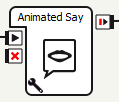
\includegraphics[width=.4\textwidth]{wrench}<1-2>
		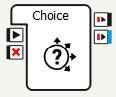
\includegraphics[width=.4\textwidth]{choice}<3->
		\end{center}
		\end{figure}
	\column{0.5\textwidth}
		\begin{itemize}
			\item<1-> Uno o più input
			\item<1-> Numero variabile di output
			\item<2-> Alcuni possono essere configurati
			\item<3-> Altri no
		\end{itemize}
\end{columns}
\end{frame}

\begin{frame}
\frametitle{Choregraphe}
\begin{figure}[ht]
\begin{center}
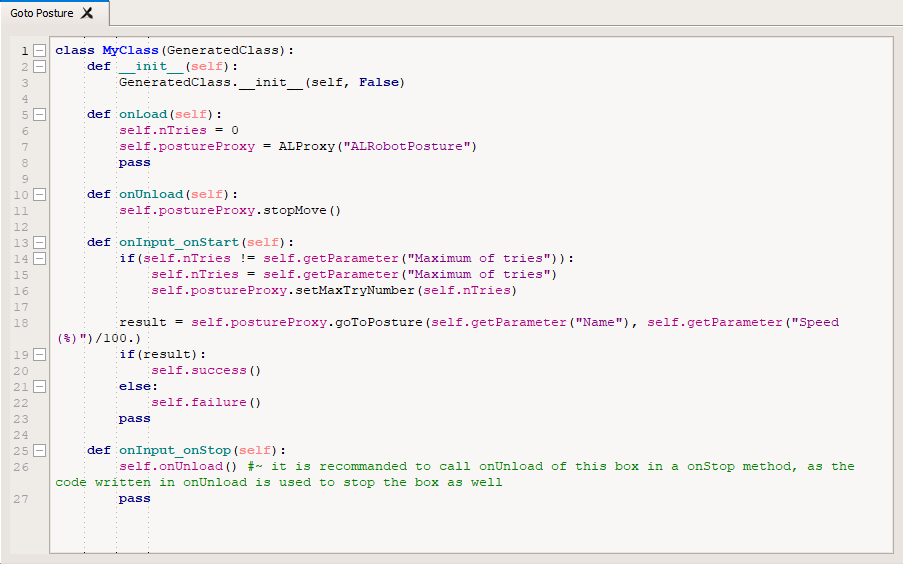
\includegraphics[width=.6\textwidth]{script}
~\footnote{Ogni blocco non è altro che un gruppo di istruzioni Python}
\end{center}
\end{figure}
\end{frame}

\section{Primo programma}

\begin{frame}
\frametitle{Choregraphe}
\begin{figure}[ht]
\begin{center}
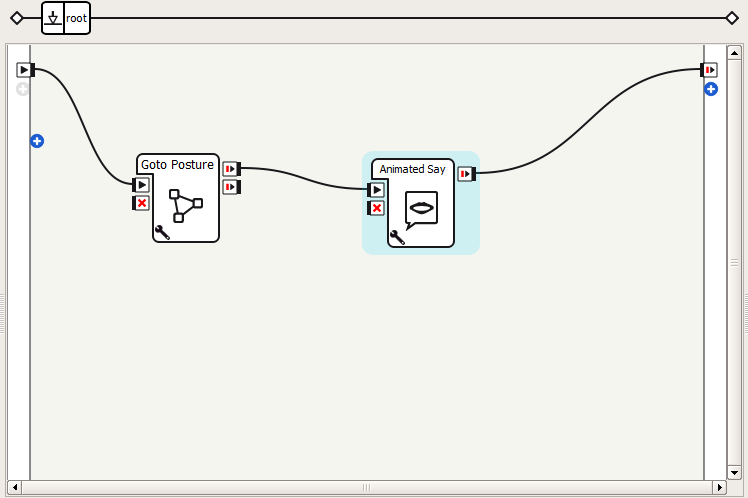
\includegraphics[width=.6\textwidth]{blocks}
~\footnote{NAO saluta con la mano}
\end{center}
\end{figure}
\end{frame}

\begin{frame}
\frametitle{Choregraphe}
\begin{figure}[ht]
\begin{center}
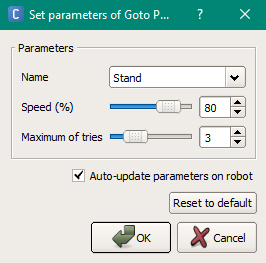
\includegraphics[width=.4\textwidth]{parameters}
~\footnote{Parametri per il blocco Goto Posture}
\end{center}
\end{figure}
\end{frame}

\begin{frame}
\frametitle{Choregraphe}
\begin{figure}[ht]
\begin{center}
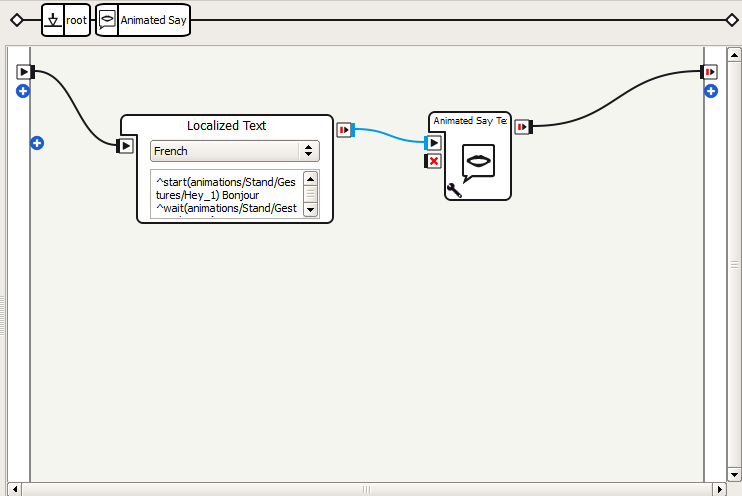
\includegraphics[width=.6\textwidth]{anisay}
~\footnote{I blocchi che compongono Animated Say}
\end{center}
\end{figure}
\end{frame}

\ifx\fulldocument\undefined
\end{document}
\fi
